\chapter{Introduzione}
\section{Storia e utilizzi della fune}
La fune è uno degli elementi costruttivi più longevo e di massivo impiego fin dal  \Rmnum{8} secolo a.C. Funi metalliche costituite da cavi di rame risalenti al 700 a.C. circa sono state ritrovate in Mesopotamia, a Babilonia, tra le rovine di Ninive (\cite{costello:fune}).

Le prime applicazioni della fune come elemento strutturale risalgono, però, al \Rmnum{15} secolo.
Basti pensare ai ponti costruiti dagli inca attraverso l'utilizzo di corde intrecciate che permettevano di superare con facilità le grandi vallate caratteristiche del territorio sudamericano (vedi figura~\ref{fig:ponte_inca}).

\begin{figure}
	\centering
	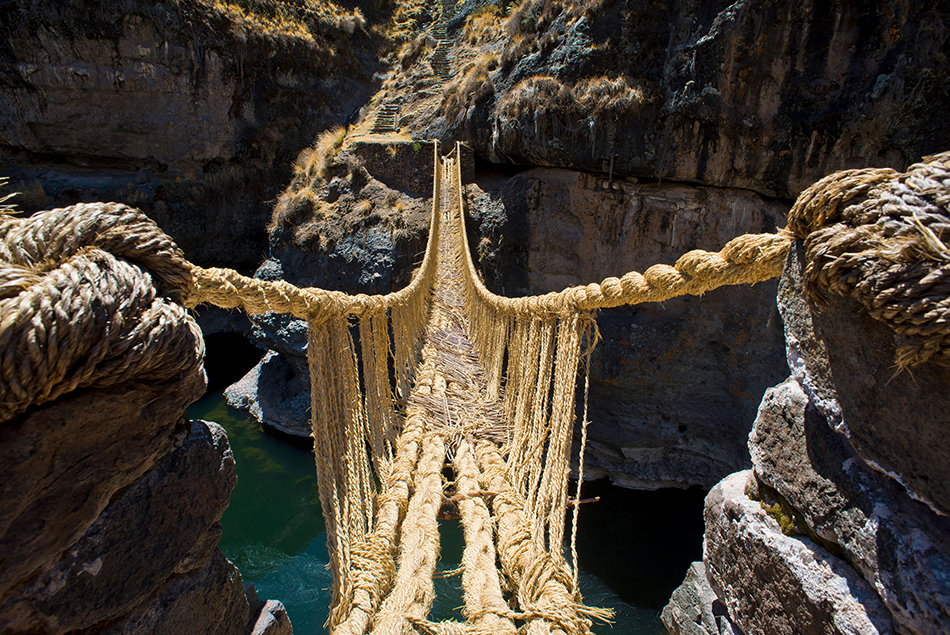
\includegraphics[width=10cm]{Immagini/Ponte_Inca}
	\caption{Ponte di corda inca sul fiume Akpurimac, Perù}	
	\label{fig:ponte_inca}
\end{figure}

Nello stesso periodo, in Tibet, Tangtong Gyalpo (1385 -- 1464) -- fisico e architetto tibetano -- costruì il primo ponte sospeso, Iron bridge (\cite{cyrus:ponte}) da cui deriva lo pseudonimo \textit{Iron Bridge Man}, sopra al fiume Kyichu, vicino a Lhasa (figura~\ref{fig:first_iron_bridge}). Questo fu il primo di una serie di ponti tibetani costruiti dal pioniere dell'ingegneria Gyalpo, principalmente localizzati nel territorio cinese.

\begin{figure}
	\centering
	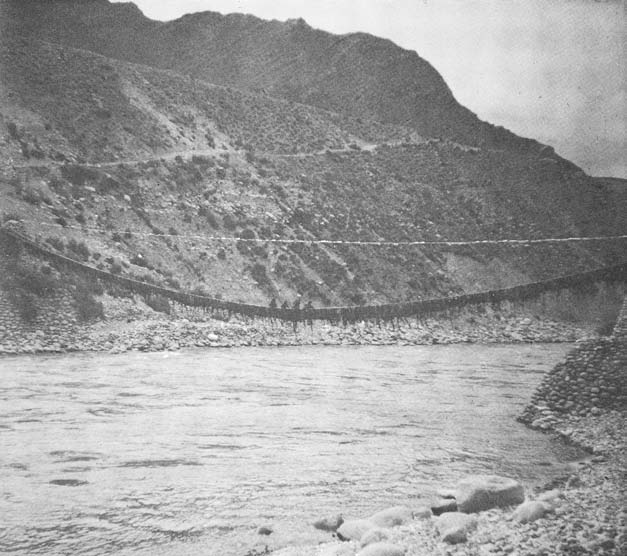
\includegraphics[width=10cm]{Immagini/Iron_Bridge_01}
	\caption{Primo ponte sospeso costruito da Gyalpo}
	\label{fig:first_iron_bridge}
\end{figure}

I ponti sospesi progettati dal fisico tibetano avevano una struttura portante formata da due lunghe catene (il cui dettaglio si può vedere in figura~\ref{fig:catena_iron_bridge}) che avevano la funzione di sorreggere, mediante altre catene, la passerella sottostante formata quasi esclusivamente da materiale ligneo (vedi figure~\ref{fig:ponte_tibetano}).

\begin{figure}
	\centering
	\subfloat[\emph{Iron bridge di Toling, Cina -- rinforzato, in seguito, da cavi in acciaio}]{
	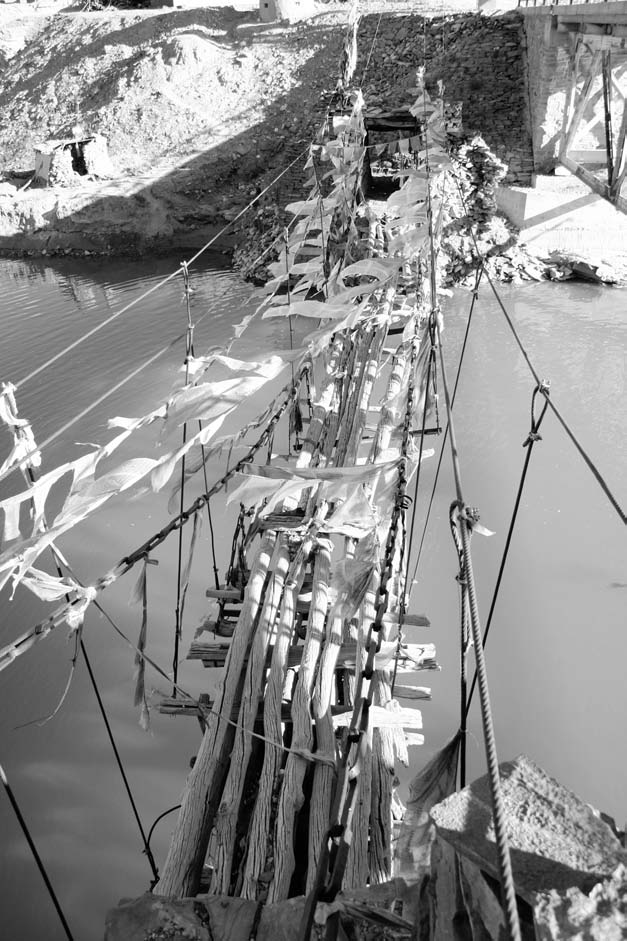
\includegraphics[width=10cm]{Immagini/Iron_Bridge}	\label{fig:iron_bridge}
}\\
	\subfloat[\emph{Catena utilizzata per la costruzione del Iron bridge}]{
	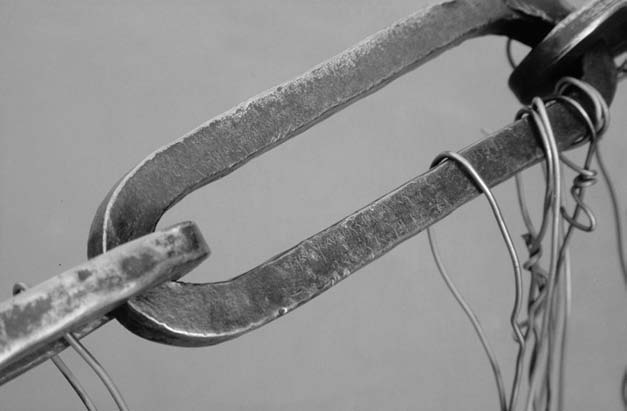
\includegraphics[width=10cm]{Immagini/Catena_Iron_Bridge}\label{fig:catena_iron_bridge}
}
	\caption{Ponte sospeso Iron bridge, Tibet}
	\label{fig:ponte_tibetano}
\end{figure}

Nonostante fossero strutture incredibili per l'epoca, questi ponti sospesi avevano una lunghezza e una portata limitata soprattutto a causa dei materiali utilizzati per la struttura portante: infatti le corde intrecciate e le catene -- benché di leghe di ferro -- non sono nemmeno paragonabili, in termini di resistenza meccanica, alle funi in uso nelle epoche successive.

Si comprende, quindi, come la consapevolezza dell'utilizzo dei cavi (intesi prima come corde e catene e in seguito come funi di acciaio)
sia da ricercarsi nell'antichità, ancora prima dello studio dello stato tensionale, risolto poi, con l'ausilio della meccanica moderna a partire da Leonardo da Vinci. 

Fu proprio da Vinci il primo a studiare la teoria delle funi, per poi essere seguito nei secoli successivi da Galileo Galilei, Huygens, Bernoulli e molti altri.
In tabella~\ref{tab:th_funi} (presa da \cite{landrini:storia}) sono riportati i contributi più significativi allo sviluppo della teoria delle funi.


\begin{table}
	\centering
	\caption{Evoluzione della teoria delle funi}
	\label{tab:th_funi}
	\begin{tabular}{p{1cm}p{3.5cm}p{5.5cm}}
		\toprule
		Anno &Autore &Oggetto\\
		\midrule
		1452 - 1519 & Leonardo da Vinci & Primi studi sulle funi\\
		1614 & Beeckman & Ponte sospeso: andamento\\&& parabolico\\
		1638 &Galileo Galilei &La parabola inestensibile\\
		1646 &Huygens &La parabola di Galileo\\&& può essere sbagliata\\
		1673 &G. Pardies &La parabola di Galileo\\&& è sbagliata\\
		1691 &Huygens, Leibniz, Bernoulli &La Catenaria inestensibile\\
		1891 &Routh &La Catenaria elastica\\
		1975 &Irvine &La Catenaria elastica sotto\\&& l'azione dei carichi concentrati	\\	
		\bottomrule
	\end{tabular}
\end{table}
%
%
%
\section{Le funi in acciaio}
Di notevole importanza per l'evoluzione della fune per uso strutturale non è solo la conoscenza matematica e fisica dettata dalla teoria dei fili, che verrà trattata nei capitoli successivi, ma è anche l'utilizzo di materiali sempre più resistenti e adatti all'uso in questione.

Ecco che si passa dall'uso di corde intrecciate e catene in ferro, all'impiego di funi in acciaio, generalmente di sezione circolare.

{\small
\begin{table}
	\centering
	\caption{Differenze tra acciaio per funi e acciaio strutturale (dolce e ad alta resistenza)\cite{gimsing:cable}}
	\label{tab:acciaio_differenze}
	\begin{tabular}{p{.21\textwidth}cccc}
		\toprule
		&Unità&Acciaio per funi&\multicolumn{2}{c}{Acciaio strutturale}\\
		&&&Dolce&Alta resistenza\\
		\midrule
		Tensione di snervamento&\si{MPa}&\num{1180}&\num{240}&\num{690}\\
		Carico di rottura a trazione&\si{MPa}&\num{1570}&\num{370}&\num{790}\\
		Deformazione a rottura&\%&\num{4}&\num{24}&-\\
		Modulo elastico&\si{GPa}&\num{205}&\num{210}&\num{210}\\
		Percentuale di carbonio presente&\%&\num{0.80}&\num{0.20}&\num{0.15}\\
		\bottomrule
	\end{tabular}
\end{table}
}

L'acciaio impiegato per le funi, a differenza di quello usato in altri ambiti, è caratterizzato da una composizione chimica con un alto contenuto di carbonio che rende la fune fino a quattro volte più resistente rispetto all'acciaio strutturale dolce\footnote{Acciaio con basso contenuto di carbonio (minore del 1\%)\cite{sito:ravaniacciai}} e fino a due volte più resistente rispetto all'acciaio ad alta resistenza rendendo, però, impossibile il collegamento dei fili mediante saldatura e creando il rischio di formazione di cricche a caldo.  

Per contro l'elevata percentuale di carbonio provoca una notevole diminuzione della duttilità del materiale riducendo a quasi un quinto la deformazione a rottura che si ha nell'acciaio strutturale dolce.

Analizzando il contenuto della tabella~\ref{tab:acciaio_differenze} della pagina successiva si evince che la resistenza a trazione dell'acciaio per funi è molto più elevata dell'acciaio per uso strutturale con un carico di rottura quasi doppio (\num{1570}\si{MPa} per la fune contro i \num{790}\si{MPa} dell'acciaio strutturale ad alta resistenza). Questa caratteristica rende la fune ideale per resistere a sforzi di trazione elevati con un impiego di materiale (e perciò di peso totale dell'opera) nettamente inferiore a strutture che impiegano altre tecnologie.
Si può notare, infine, una diminuzione del modulo elastico che passa da \num{210}\si{GPa} a \num{205}\si{GPa} il quale implica che, a parità di sforzo impresso, la deformazione aumenta (linearmente in caso di campo elastico -- lineare).

La versatilità della fune sta principalmente nel fatto di essere prefabbricata e quindi componibile a piacere: in base al diametro di cui si necessita è possibile assemblare la fune mediante l'insieme di fili.

\begin{figure}[t]
	\centering
	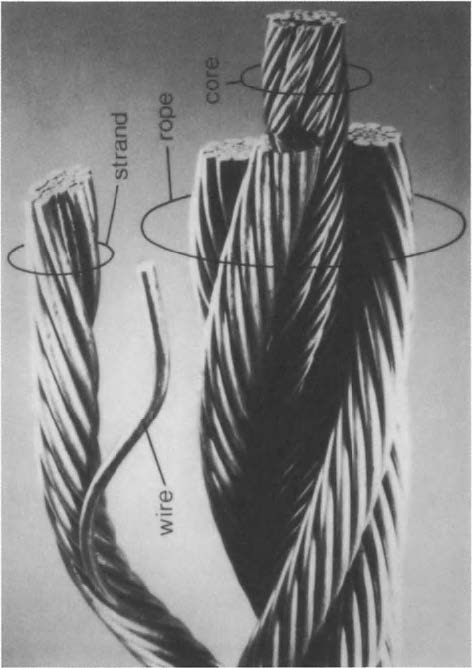
\includegraphics[width=10cm]{Immagini/Fune}
	\caption{Composizione di una fune di acciaio (\cite{costello:fune})}
	\label{fig:fune}
\end{figure}

In particolare, come descritto in figura~\ref{fig:fune}, la fune è composta come segue:
\begin{enumerate}
	\item filo (\textit{wire}): elemento base per la composizione della fune;
	\item trefolo (\textit{strand}): insieme di fili disposti in svariate forme;
	\item fune (\textit{rope}): elemento finale composto da un determinato numero di trefoli avvolti elicoidalmente attorno a un'anima centrale (\textit{core}) che può essere a sua volta un trefolo.
\end{enumerate}

\subsection{Filo}
Il filo è l'elemento alla base della fune. In base alle applicazioni il diametro del filo può variare; ad esempio, per le funi usate nei ponti moderni si possono trovare diametri di:
\begin{itemize}
	\item \num{5}\,--\,\num{5.5}\si{mm} per i cavi principali dei ponti sospesi;
	\item \num{7}\si{mm} per i cavi di ponti strallati.
\end{itemize}


\subsection{Trefolo}
Il trefolo è un insieme di fili in opportune configurazioni: i fili possono essere avvolti elicoidalmente oppure disposti in maniera parallela.
%In ambito strutturale si usa una configurazione di sette fili da \num{5}\si{mm} per un diametro nominale del trefolo di \num{15}\si{mm};

\begin{figure}[]
	\centering
	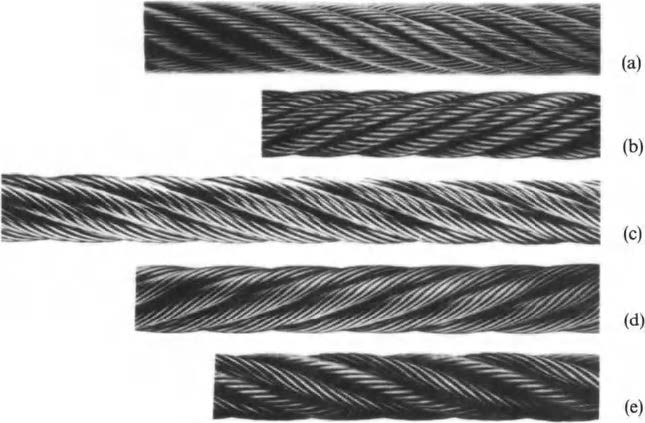
\includegraphics[width=10cm]{Immagini/Avvolgimento_Trefolo}
	\caption{Tipologie di avvolgimento dei fili che formano il trefolo [\cite{costello:fune}]}
	\label{fig:avvolgimento_trefolo}
\end{figure}

\subsubsection*{Avvolgimento elicoidale}
Per quanto riguarda l'avvolgimento elicoidale ne esistono di vari tipi: in figura~\ref{fig:avvolgimento_trefolo} sono mostrati i principali.

In particolare si differenziano tra loro per la posa (\textit{lay}) che descrive il senso di rotazione dei fili durante la costruzione del trefolo (\textit{right} o \textit{left}) e per la direzione di posa dei fili rispetto a quella del trefolo; questa può essere crociata (\textit{regular}) se i fili che compongono il trefolo sono posati nel senso opposto ai trefoli che compongono la fune oppure parallela (\textit{lang}) se i fili sono posati nello stesso verso del trefolo.

In dettaglio si ha:
\begin{description}[font=\normalfont]
	\item[(a)] \emph{Right regular lay:} i fili sono avvolti in modo tale da andare da sinistra verso destra (\textit{right}) e sono posati con senso opposto rispetto alla posa del trefolo (\textit{regular});
	\item [(b)] \emph{Left regular lay:} i fili sono avvolti da destra verso sinistra (\textit{left}) e hanno direzione opposta al trefolo (\textit{regular});
	\item [(c)] \emph{Right lang lay:} l'avvolgimento va da sinistra a destra (\textit{right}). I fili sono posati in modo concorde al senso di posa del trefolo (\textit{lang});
	\item [(d)] \emph{Left lang lay:} l'avvolgimento va da destra verso sinistra (\textit{left}). La posa avviene in maniera concorde al trefolo (\textit{lang});
	\item[(e)] \emph{Right alternate lay:} i fili hanno verso da sinistra a destra (\textit{right}) mentre la posa viene alternata tra \textit{regular} e \textit{lang}.
\end{description}
La cordatura \textit{right regular}, grazie alla posa crociata, è meno soggetta a torsioni e schiacciamenti ed è quindi la posa adatta alla maggior parte delle applicazioni.
La cordatura \textit{lang}, invece, ha una flessibilità maggiore e quindi si può flettere più facilmente, a parità di diametro, rispetto alla precedente tipologia. Tende, inoltre, a collassare in caso di eccessive rotazioni, il che la rende meno adatta per applicazioni strutturali.

In alternativa si possono sovrapporre diversi strati di fili avvolti elicoidalmente la cui anima centrale è un unico filo rettilineo.

Poiché sono presenti spazi vuoti nell'avvolgimento, quando il carico viene applicato alla fune si ha un assestamento dei trefoli che genera una deformazione irreversibile. Per questo motivo prima dell'applicazione del carico viene effettuato un pretensionamento che ha il fine di compattare il cavo e risolvere il problema sopra descritto.

%%%%%%%%%%%%%%%%%%%%%%%%%%%%%%%%%%%%%%%%%%%%%%%%%%%%%%%%%%%%%%%%%%%%%%%%



%%%%%%%%%%%%%%%%%%%%%%%%%%%%%%%%%%%%%%%%%%%%%%%%%%%%%%%%%%%%%%%%%%%%%%%%

\subsubsection*{Locked--coil strands}
Il locked--coil strand è una tipologia di trefolo formata da due diversi tipi di fili avvolti elicoidalmente. L'anima centrale è un trefolo generico, composto da due o più strati di fili che si avvolgono ellitticamente con le pose viste sopra.
All'esterno sono posti dei particolari fili a forma di \textit{Z} che si incastrano perfettamente, diminuendo di molto gli interstizi (minori del \num{10}\%) e di conseguenza aumentando la superficie di contatto che risulta molto più continua e compatta rispetto alle altre tipologie. Questo protegge maggiormente il trefolo dalla corrosione e lo rende più resistente a pressioni laterali.

\begin{figure}
	\centering
	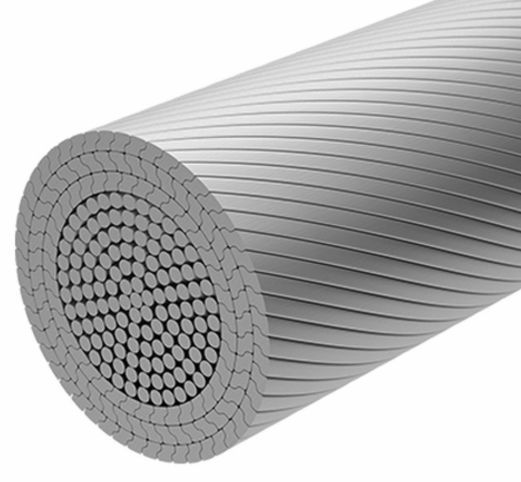
\includegraphics[width=9cm]{Immagini/Locked_coil_strands}
	\caption{Esempio di locked--coil strand}
	\label{fig:locked_coil_strands}
\end{figure}

\subsubsection*{Parallel--wire strands}
Per via della diminuzione di resistenza e rigidezza a cui sono soggette le funi ellittiche, sono stati sviluppati dei particolari trefoli composti da soli fili paralleli tra loro.

Inizialmente questa tipologia portava con se una problematica che rendeva il trefolo inutilizzabile: l'avvolgimento. Infatti, per evitare distorsioni sulla sezione durante l'avvolgimento si sarebbe dovuto avere un allungamento dei fili superiori e un accorciamento dei fili interni alla curva che, però, avrebbe generato nel materiale delle tensioni molto elevate e quindi non ammissibili.

In figura~\ref{fig:parallel_wire_strands} sono descritti i principali tipi di \emph{parallel--wire strands}; in particolare, partendo da sinistra si ha:
\begin{itemize}
	\item \emph{Regular Hexagonal}: i fili sono disposti in modo da formare un cavo di forma esagonale;
	\item \emph{Deformed Hexagonal}: rispetto a quello precedente risulta più "schiacciato" in altezza;
	\item \emph{Quasi Hexagonal}: ha una forma simile a un esagono.
\end{itemize}

In tutti i casi sopra descritti vengono impiegati fili di diametro \num{5}\si{mm}.

\begin{figure}
	\centering
	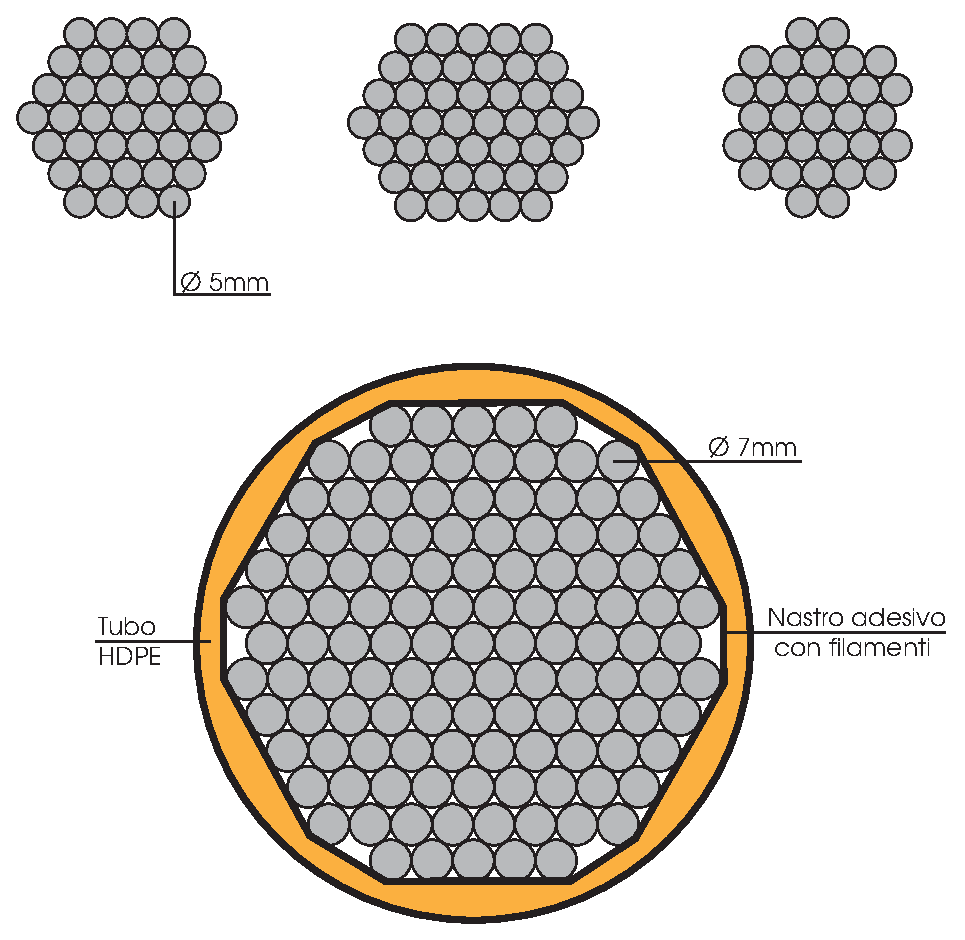
\includegraphics[width=10cm]{Immagini/Parallel_wire_strands}
	\caption{Esempi di \emph{parallel--wire strands} (in alto) e \emph{new PWS cable} (in basso)}
	\label{fig:parallel_wire_strands}
\end{figure}

Nel tempo sono state proposte varie soluzioni al problema, una delle quali è quella di inserire i fili in un involucro di polietilene (HDPE -- High Density Poly-Ethylene) che evita rotazioni e deformazioni della sezione in modo che questa mantenga la forma originale. Questa soluzione prende il nome di \emph{New PWS Cable} ed è stata sviluppata in Giappone negli anni '90. In figura~\ref{fig:parallel_wire_strands} (in basso) è rappresentata una sezione del cavo \textit{PWS}.
%*************************************************
%************************************************
%*********************************************
\section{Applicazione delle funi a strutture moderne}
L'avvento dell'acciaio consente, grazie alla sua miglior resistenza meccanica, di costruire strutture molto snelle e di lunghezze in precedenza impensabili.
In particolare, i ponti moderni che impiegano le funi possono essere classificati in:
\begin{enumerate}
	\item ponti sospesi;
	\item ponti strallati.
\end{enumerate}

Questi si differenziano tra loro principalmente per la configurazione del sistema di funi che crea una diversificazione nelle applicazioni, in particolare nella lunghezza delle campate.

\subsection{Ponti sospesi}
I ponti sospesi sono, tra i ponti moderni, quelli che collegano distanze elevate (200 -- 2000\si{m}), motivo per cui sono largamente utilizzati sia in ambito stradale che in ambito ferroviario. 

\begin{figure}
	\centering
	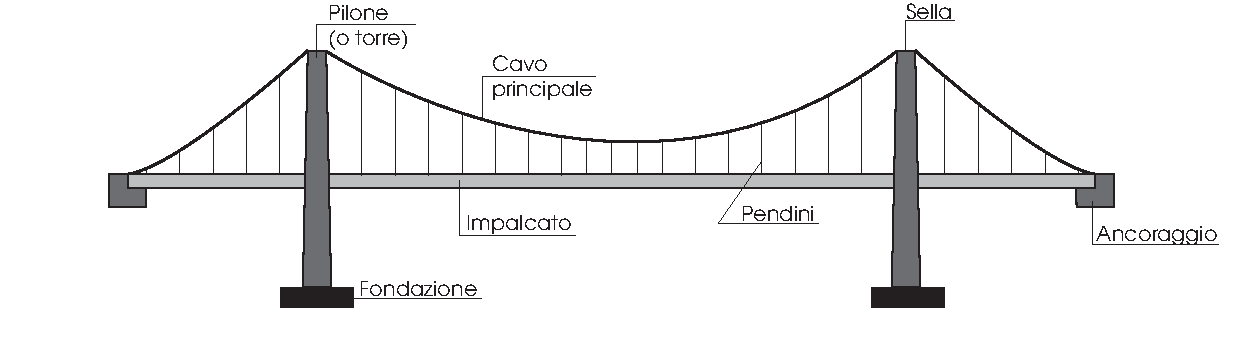
\includegraphics[width=11.8cm, keepaspectratio]{Immagini/suspension_bridge}
	\caption{Schema di un ponte sospeso}
	\label{fig:ponte_sospeso}
\end{figure}
\begin{figure}
	\centering
	
	\begin{tikzpicture}
	
	%\draw[help lines] (0,0) grid (10,5);
	\point {a}{0}{2};
	\point {b}{1}{2};
	\point {c}{2}{0};
	\point {d}{8}{0};
	\point {e}{9}{2};
	\point {f}{10}{2};
	\point {g}{8}{5};
	\point {h}{2}{5};
	
	\beam {2}{a}{h};
	\beam {2}{b}{e};
	\beam {2}{c}{h};
	\beam {2}{d}{g};
	\beam {2}{f}{g};
	
	\support {1}{b};
	\support {1}{e};
	\support {3}{c};
	\support {3}{d};
	\support {3}{a}[-45];
	\support {3}{f}[45];
	
	\internalforces{h}{g}{0}{0}[-2.5][black];

	
	
	
	
	
	
	\end{tikzpicture}
	
	
	\caption{Schema statico di un ponte sospeso}
	\label{fig:schema_statico_sospeso}
	
\end{figure}

Come descritto in figura~\ref{fig:ponte_sospeso} i ponti sospesi si compongono di:
\begin{itemize}
	\item impalcato: parte transitabile della struttura che può essere in acciaio o cemento armato e può essere pedonale, ferroviaria o stradale. L'impalcato ha anch'esso un compito di resistenza essendo dotato di rigidezza flessionale che riduce così le deformazioni del piano;
	\item sistema di cavi: elemento caratteristico dei ponti sospesi, comprende il cavo principale e i pendini (cavi verticali) e ha il compito di trasmettere gli sforzi dall'impalcato alle torri. Sotto l'effetto della forza peso tende ad acquisire una forma simile a una parabola;
	\item piloni (o torri): elementi che scaricano gli sforzi derivanti dalle funi  alle fondazioni e quindi al terreno. Sono soggetti a momento flettente, motivo per cui il cavo principale viene fatto proseguire e vincolato in appositi ancoraggi a terra. In questo modo il momento flettente generato viene equilibrato;
\end{itemize}

Difficilmente le campate risultano tutte di egual misura; infatti si predilige l'impiego di una campata centrale molto lunga e due campate laterali di lunghezza inferiore.
Nel caso di campate laterali di lunghezza uguale si otterrebbe una struttura simmetrica; ma in molti casi queste hanno lunghezze differenti dipendenti dalla morfologia del territorio.

\subsection{Ponti strallati}

\begin{figure}
	\centering
	\subfloat[\emph{Schema a ventaglio}]{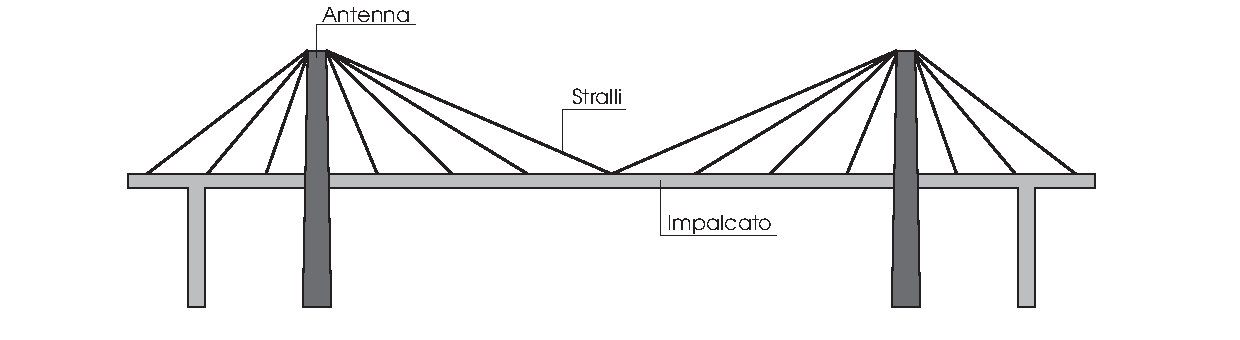
\includegraphics[width=11.8cm]{Immagini/cable_stayed_bridge_ventaglio}\label{fig:cable_stayed_ventaglio}}\\
	\subfloat[\emph{Schema a semi--ventaglio o "ventaglio modificato"}]{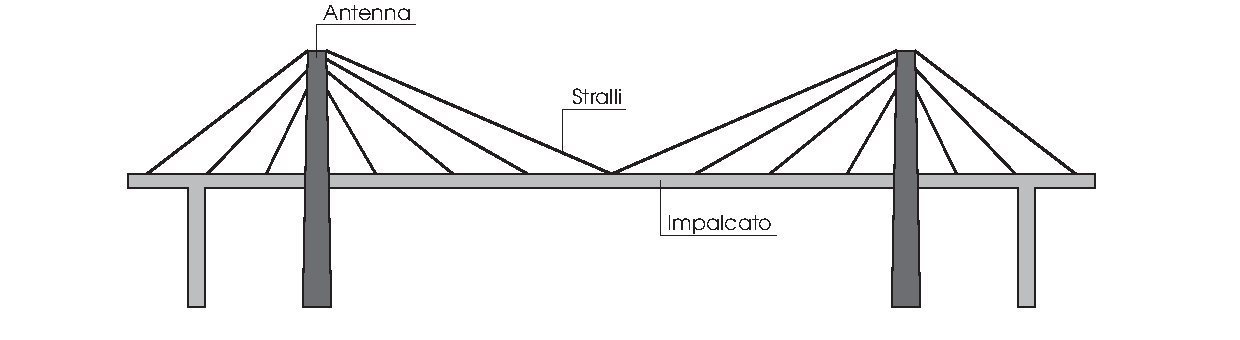
\includegraphics[width=11.8cm]{Immagini/cable_stayed_bridge_semiventaglio}\label{fig:cable_stayed_semiventaglio}}\\
	\subfloat[\emph{Schema ad arpa}]{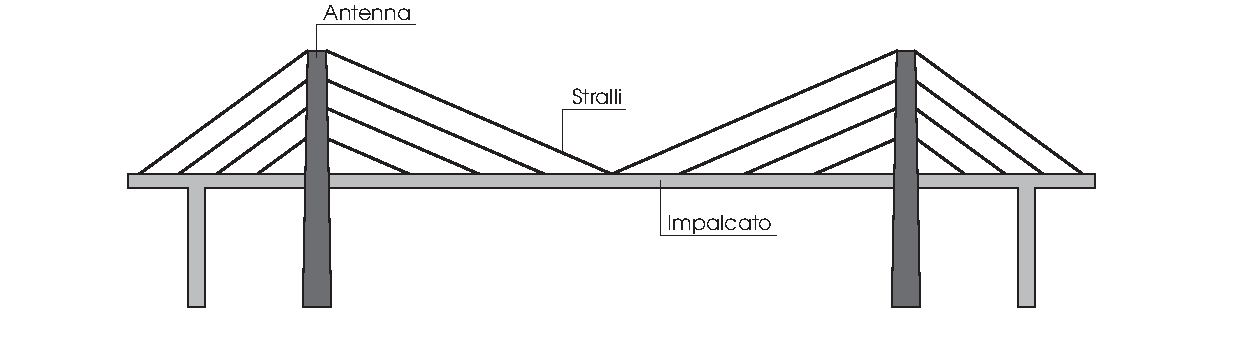
\includegraphics[width=11.8cm]{Immagini/cable_stayed_bridge_arpa}\label{fig:cable_stayed_arpa}}
	\caption{Schemi delle varie tipologie di ponti strallati}
	\label{fig:cable_stayed_bridge}
\end{figure}

\begin{figure}
	\centering
	
	\begin{tikzpicture}
	\scaling{.58};
	
	\point {a}{-5}{4};
	\point {b}{5}{4};
	\point {c}{-9}{0};
	\point {d}{9}{0};
	\point {e}{-9}{-2};
	\point {f}{9}{-2};
	
	
	\point {g2}{-8}{0};
	\point {g3}{-7}{0};
	\point {g4}{-6}{0};
	\point {g5}{-5}{-2};
	\point {g6}{-4}{0};
	\point {g7}{-3}{0};
	\point {g8}{-2}{0};
	\point {g9}{-1}{0};
	
	\point {h1}{1}{0};
	\point {h2}{2}{0};
	\point {h3}{3}{0};
	\point {h4}{4}{0};
	\point {h5}{5}{-2};
	\point {h6}{6}{0};
	\point {h7}{7}{0};
	\point {h8}{8}{0};
	
	
	\beam {2}{c}{d};
	
	\beam {2}{a}{c};
	\beam {2}{c}{e};
	\beam {2}{b}{d};
	\beam {2}{d}{f};
	\beam {2}{a}{g9};
	\beam {2}{b}{h1};
	\beam {2}{a}{g2};
	\beam {2}{a}{g3};
	\beam {2}{a}{g4};
	\beam {2}{a}{g5};
	\beam {2}{a}{g6};
	\beam {2}{a}{g7};
	\beam {2}{a}{g8};
	\beam {2}{b}{h1};
	\beam {2}{b}{h2};
	\beam {2}{b}{h3};
	\beam {2}{b}{h4};
	\beam {2}{b}{h5};
	\beam {2}{b}{h6};
	\beam {2}{b}{h7};
	\beam {2}{b}{h8};
	
	\support {1}{e};
	\support {1}{f};
	\support {3}{g5};
	\support {3}{h5};
	
	\hinge {1}{a};
	\hinge {1}{b};
	\hinge {1}{c};
	\hinge {1}{d};
	\hinge {1}{e};
	\hinge {1}{f};
	\hinge {1}{g2};
	\hinge {1}{g3};
	\hinge {1}{g4};
	%\hinge {1}{g5};
	\hinge {1}{g6};
	\hinge {1}{g7};
	\hinge {1}{g8};
	\hinge {1}{g9};
	
	\hinge {1}{h1};
	\hinge {1}{h2};
	\hinge {1}{h3};
	\hinge {1}{h4};
	%\hinge {1}{h5};
	\hinge {1}{h6};
	\hinge {1}{h7};
	\hinge {1}{h8};
	\end{tikzpicture}
		
	
	\caption{Schema statico di un ponte strallato a ventaglio}
	\label{fig:schema_statico_ventaglio}
\end{figure}

In epoca moderna i ponti strallati sono i più usati per congiungere punti posti a distanze medio -- lunghe (intorno ai 1000\si{m}).
Si differenziano, dai ponti sospesi, in maniera molto chiara per il sistema di cavi, detti \emph{stralli}, che - una volta posati - risultano quasi rettilinei.

In questa configurazione l'impalcato è sorretto dagli stralli, che risultano soggetti a uno sforzo di trazione e inducono uno stato di compressione nella torre e nell'impalcato.

La compressione che si genera nell'impalcato provoca l'impossibilità di raggiungere luci elevate con questa tipologia di ponte. Per colmare, in parte, il problema è consigliato ancorare gli stralli di riva a terra in modo da limitare il carico sull'impalcato.



In figura~\ref{fig:cable_stayed_bridge} sono rappresentate le diverse configurazioni degli stralli; infatti, in base al collegamento dei cavi con la torre si possono ottenere diverse tipologie di ponti strallati.
\subsubsection{Schema a ventaglio}

Nel caso in cui i cavi convergano in un solo punto alla sommità della torre si parla di \emph{schema a ventaglio} (figura~\ref{fig:cable_stayed_ventaglio}).

Questa disposizione risulta molto efficiente grazie al fatto che avvicinandosi alla torre l'angolo compreso tra l'impalcato e lo strallo aumenta; ne consegue che la componente orizzontale degli sforzi assorbita dall'impalcato diminuisce. 

Per motivi tecnici, in presenza di molti stralli, risulta difficoltoso ancorare i cavi disposti a ventaglio alla torre. Per questo si utilizza lo schema a \emph{semi--ventaglio}.

\subsubsection{Schema a semi--ventaglio}
Usato nel caso di un numero elevato di cavi, è simile allo schema a ventaglio, mantenendone le particolarità positive e risolvendo il problema dell'ancoraggio andando a distribuire l'attacco degli stralli nella parte superiore della torre (come si può vedere in figura~\ref{fig:cable_stayed_semiventaglio}).

\subsubsection{Schema ad arpa}
La disposizione ad arpa (figura~\ref{fig:cable_stayed_arpa}) è composta da stralli tutti paralleli tra loro, implicando così, la distribuzione degli ancoraggi lungo tutta la torre.
Le distanze tra gli ancoraggi verticali e orizzontali sono tra loro proporzionali.
Questo schema è quello meno efficiente tra quelli visti poiché il sistema di cavi paralleli genera uno stato tensionale di compressione notevole nell'impalcato che lo rende non adatto a coprire luci elevate.







 


